\chapter{Geometria}

\index{geometria}

Geometrian tehtävissä on usein haasteena keksiä,
mistä suunnasta ongelmaa kannattaa lähestyä,
jotta ratkaisun saa koodattua mukavasti ja
erikoistapauksia tulee mahdollisimman vähän.

Tarkastellaan esimerkkinä tehtävää,
jossa annettuna on nelikulmion kulmapisteet
ja tehtävänä on laskea sen pinta-ala.
Esimerkiksi syötteenä voi olla
seuraavanlainen nelikulmio:

\begin{center}
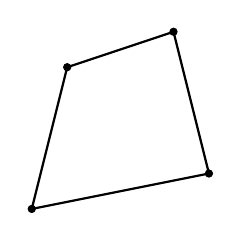
\begin{tikzpicture}[scale=0.45]

\draw[fill] (6,2) circle [radius=0.1];
\draw[fill] (5,6) circle [radius=0.1];
\draw[fill] (2,5) circle [radius=0.1];
\draw[fill] (1,1) circle [radius=0.1];
\draw[thick] (6,2) -- (5,6) -- (2,5) -- (1,1) -- (6,2);
\end{tikzpicture}
\end{center}
Yksi tapa lähestyä tehtävää on jakaa nelikulmio
kahdeksi kolmioksi vetämällä jakoviiva kahden
vastakkaisen kulmapisteen välille:
\begin{center}
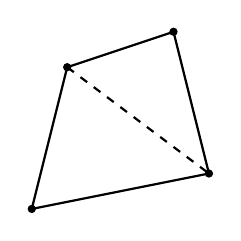
\begin{tikzpicture}[scale=0.45]

\draw[fill] (6,2) circle [radius=0.1];
\draw[fill] (5,6) circle [radius=0.1];
\draw[fill] (2,5) circle [radius=0.1];
\draw[fill] (1,1) circle [radius=0.1];

\draw[thick] (6,2) -- (5,6) -- (2,5) -- (1,1) -- (6,2);
\draw[dashed,thick] (2,5) -- (6,2);
\end{tikzpicture}
\end{center}
Tämän jälkeen riittää laskea yhteen kolmioiden
pinta-alat. Kolmion pinta-alan voi laskea
esimerkiksi Heronin kaavalla
\[ \sqrt{s (s-a) (s-b) (s-c)},\]
kun kolmion sivujen pituudet ovat
$a$, $b$ ja $c$ ja $s=(a+b+c)/2$.
\index{Heronin kaava}

Tämä on mahdollinen tapa ratkaista tehtävä,
mutta siinä on ongelma:
miten löytää kelvollinen tapa vetää jakoviiva?
Osoittautuu, että
mitkä tahansa vastakkaiset pisteet eivät kelpaa.
Esimerkiksi seuraavassa nelikulmiossa
jakoviiva menee nelikulmion ulkopuolelle:
\begin{center}
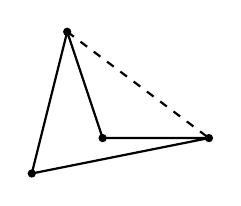
\begin{tikzpicture}[scale=0.45]

\draw[fill] (6,2) circle [radius=0.1];
\draw[fill] (3,2) circle [radius=0.1];
\draw[fill] (2,5) circle [radius=0.1];
\draw[fill] (1,1) circle [radius=0.1];
\draw[thick] (6,2) -- (3,2) -- (2,5) -- (1,1) -- (6,2);

\draw[dashed,thick] (2,5) -- (6,2);
\end{tikzpicture}
\end{center}
Toinen tapa vetää jakoviiva on kuitenkin toimiva:
\begin{center}
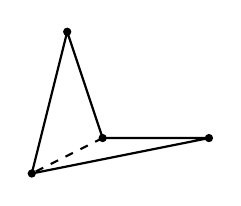
\begin{tikzpicture}[scale=0.45]

\draw[fill] (6,2) circle [radius=0.1];
\draw[fill] (3,2) circle [radius=0.1];
\draw[fill] (2,5) circle [radius=0.1];
\draw[fill] (1,1) circle [radius=0.1];
\draw[thick] (6,2) -- (3,2) -- (2,5) -- (1,1) -- (6,2);

\draw[dashed,thick] (3,2) -- (1,1);
\end{tikzpicture}
\end{center}
Ihmiselle on selvää, kumpi jakoviiva jakaa nelikulmion
kahdeksi kolmioksi, mutta tietokoneen kannalta
tilanne on hankala.

Osoittautuu, että tehtävän ratkaisuun on olemassa
paljon helpommin toteutettava tapa,
jossa ei tarvitse miettiä erikoistapauksia.
Nelikulmion pinta-alan laskemiseen
on nimittäin yleinen kaava
\[x_1y_2-x_2y_1+x_2y_3-x_3y_2+x_3y_4-x_4y_3+x_4y_1-x_1y_4,\]
kun kulmapisteet ovat
$(x_1,y_1)$,
$(x_2,y_2)$,
$(x_3,y_3)$ ja
$(x_4,y_4)$.
Tämä kaava on helppo laskea, siinä ei ole erikoistapauksia
ja osoittautuu, että kaava on mahdollista yleistää
\textit{kaikille} monikulmioille.

\section{Kompleksiluvut}

\index{kompleksiluku}
\index{piste}
\index{vektori}

Kompleksiluku on luku muotoa $x+y i$, missä $i = \sqrt{-1}$
on imaginääriyksikkö.
Kompleksiluvun luonteva geometrinen tulkinta on,
että se esittää kaksiulotteisen tason pistettä $(x,y)$
tai vektoria origosta pisteeseen $(x,y)$.

Esimerkiksi luku $4+2i$ tarkoittaa seuraavaa
pistettä ja vektoria:

\begin{center}
\begin{tikzpicture}[scale=0.45]

\draw[->,thick] (-5,0)--(5,0);
\draw[->,thick] (0,-5)--(0,5);

\draw[fill] (4,2) circle [radius=0.1];
\draw[->,thick] (0,0)--(4-0.1,2-0.1);

\node at (4,2.8) {$(4,2)$};
\end{tikzpicture}
\end{center}

\index{\texttt{complex}}

C++:ssa on kompleksilukujen käsittelyyn luokka \texttt{complex},
josta on hyötyä geometriassa.
Luokan avulla voi esittää pisteen tai vektorin
kompleksilukuna, ja luokassa on valmiita
geometriaan soveltuvia työkaluja.

Seuraavassa koodissa \texttt{C} on koordinaatin tyyppi
ja \texttt{P} on pisteen tai vektorin tyyppi.
Lisäksi koodi määrittelee
lyhennysmerkinnät \texttt{X} ja \texttt{Y},
joiden avulla pystyy viittaamaan x- ja y-koordinaatteihin.

\begin{lstlisting}
typedef long long C;
typedef complex<C> P;
#define X real()
#define Y imag()
\end{lstlisting}

Esimerkiksi seuraava koodi määrittelee pisteen $p=(4,2)$
ja ilmoittaa sen x- ja y-koordinaatin:

\begin{lstlisting}
P p = {4,2};
cout << p.X << " " << p.Y << "\n"; // 4 2
\end{lstlisting}

Seuraava koodi määrittelee vektorit $v=(3,1)$
ja $u=(2,2)$ ja laskee sitten niiden summan $s=v+u$:

\begin{lstlisting}
P v = {3,1};
P u = {2,2};
P s = v+u;
cout << s.X << " " << s.Y << "\n"; // 5 3
\end{lstlisting}

Sopiva koordinaatin tyyppi \texttt{C} on tilanteesta
riippuen \texttt{long long} (kokonaisluku)
tai \texttt{long double} (liukuluku).
Kokonaislukuja kannattaa käyttää aina kun mahdollista,
koska silloin laskenta on tarkkaa.

Jos koordinaatit ovat liukulukuja,
niiden vertailussa täytyy ottaa huomioon epätarkkuus.
Turvallinen tapa tarkistaa,
ovatko liukuluvut $a$ ja $b$ samat
on käyttää vertailua $|a-b|<\epsilon$, jossa $\epsilon$
on pieni luku (esimerkiksi $\epsilon=10^{-9}$).

\subsubsection*{Funktioita}

Seuraavissa esimerkeissä koordinaatin tyyppinä on
\texttt{long double}.

Funktio \texttt{abs(v)} laskee vektorin $v=(x,y)$
pituuden $|v|$ kaavalla $\sqrt{x^2+y^2}$.
Sillä voi laskea myös pisteiden $(x_1,y_1)$
ja $(x_2,y_2)$ etäisyyden,
koska pisteiden etäisyys
on sama kuin vektorin $(x_2-x_1,y_2-y_1)$ pituus.
Joskus hyödyllinen on myös funktio \texttt{norm(v)},
joka laskee vektorin $v=(x,y)$ pituuden neliön $|v|^2$.

Seuraava koodi laskee
pisteiden $(4,2)$ ja $(3,-1)$ etäisyyden:
\begin{lstlisting}
P a = {4,2};
P b = {3,-1};
cout << abs(b-a) << "\n"; // 3.60555
\end{lstlisting}

Funktio \texttt{arg(v)} laskee vektorin $v=(x,y)$
kulman radiaaneina suhteessa x-akseliin.
Radiaaneina ilmoitettu kulma $r$ vastaa asteina
kulmaa $180  r/\pi$ astetta.
Jos vektori osoittaa suoraan oikealle,
sen kulma on 0.
Kulma kasvaa vastapäivään ja vähenee myötäpäivään
liikuttaessa.

Funktio \texttt{polar(s,a)} muodostaa vektorin,
jonka pituus on $s$ ja joka osoittaa kulmaan $a$.
Lisäksi vektoria pystyy kääntämään kulman $a$
verran kertomalla se vektorilla,
jonka pituus on 1 ja kulma on $a$.

Seuraava koodi laskee vektorin $(4,2)$ kulman,
kääntää sitä sitten $1/2$ radiaania vastapäivään
ja laskee uuden kulman:

\begin{lstlisting}
P v = {4,2};
cout << arg(v) << "\n"; // 0.463648
v *= polar(1.0,0.5);
cout << arg(v) << "\n"; // 0.963648
\end{lstlisting}

\section{Pisteet ja suorat}

\index{ristitulo}
Vektorien
$a=(x_1,y_1)$ ja $b=(x_2,y_2)$ ristitulo $a \times b$
lasketaan kaavalla $x_1 y_2 - x_2 y_1$.
Ristitulo ilmaisee, mihin suuntaan vektori $b$
kääntyy, jos se laitetaan vektorin $a$ perään.
Positiivinen ristitulo tarkoittaa käännöstä vasemmalle,
negatiivinen käännöstä oikealle, ja nolla tarkoittaa,
että vektorit ovat samalla suoralla.

Seuraava kuva näyttää kolme esimerkkiä ristitulosta:
\begin{center}
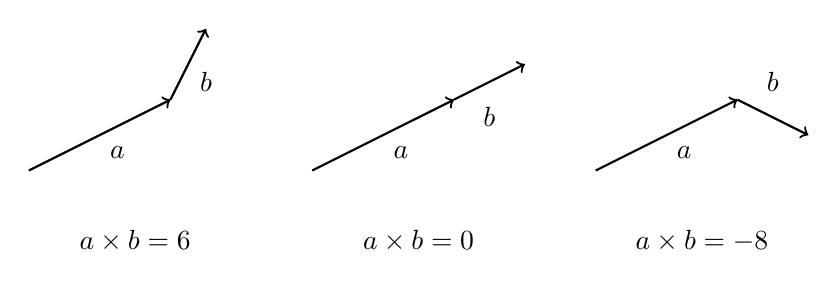
\begin{tikzpicture}[scale=0.45]

\draw[->,thick] (0,0)--(4,2);
\draw[->,thick] (4,2)--(4+1,2+2);

\node at (2.5,0.5) {$a$};
\node at (5,2.5) {$b$};

\node at (3,-2) {$a \times b = 6$};

\draw[->,thick] (8+0,0)--(8+4,2);
\draw[->,thick] (8+4,2)--(8+4+2,2+1);

\node at (8+2.5,0.5) {$a$};
\node at (8+5,1.5) {$b$};

\node at (8+3,-2) {$a \times b = 0$};

\draw[->,thick] (16+0,0)--(16+4,2);
\draw[->,thick] (16+4,2)--(16+4+2,2-1);

\node at (16+2.5,0.5) {$a$};
\node at (16+5,2.5) {$b$};

\node at (16+3,-2) {$a \times b = -8$};
\end{tikzpicture}
\end{center}

\noindent
Esimerkiksi vasemmassa kuvassa
$a=(4,2)$ ja $b=(1,2)$.
Seuraava koodi laskee vastaavan ristitulon
luokkaa \texttt{complex} käyttäen:

\begin{lstlisting}
P a = {4,2};
P b = {1,2};
C r = (conj(a)*b).Y; // 6
\end{lstlisting}

Tämä perustuu siihen, että funktio \texttt{conj}
muuttaa vektorin y-koordinaatin käänteiseksi
ja kompleksilukujen kertolaskun seurauksena
vektorien $(x_1,-y_1)$ ja $(x_2,y_2)$
kertolaskun y-koordinaatti on $x_1 y_2 - x_2 y_1$.

\subsubsection{Pisteen sijainti suoraan nähden}

Ristitulon avulla voi selvittää,
kummalla puolella suoraa tutkittava piste sijaitsee.
Oletetaan, että suora kulkee pisteiden
$s_1$ ja $s_2$ kautta, katsontasuunta on
pisteestä $s_1$ pisteeseen $s_2$ ja
tutkittava piste on $p$.

Esimerkiksi seuraavassa kuvassa piste $p$
on suoran vasemmalla puolella:
\begin{center}
\begin{tikzpicture}[scale=0.45]
\draw[dashed,thick,->] (0,-3)--(12,6);
\draw[fill] (4,0) circle [radius=0.1];
\draw[fill] (8,3) circle [radius=0.1];
\draw[fill] (5,3) circle [radius=0.1];
\node at (4,-1) {$s_1$};
\node at (8,2) {$s_2$};
\node at (5,4) {$p$};
\end{tikzpicture}
\end{center}

Nyt ristitulo $(p-s_1) \times (p-s_2)$
kertoo, kummalla puolella suoraa piste $p$ sijaitsee.
Jos ristitulo on positiivinen,
piste $p$ on suoran vasemmalla puolella,
ja jos ristitulo on negatiivinen,
piste $p$ on suoran oikealla puolella.
Jos taas ristitulo on nolla,
piste $p$ on pisteiden $s_1$ ja $s_2$
kanssa suoralla.

\subsubsection{Janojen leikkaaminen}

Tarkastellaan tilannetta, jossa tasossa on kaksi
janaa $ab$ ja $cd$ ja tehtävänä on selvittää,
leikkaavatko janat. Mahdolliset tapaukset ovat seuraavat:

\textit{Tapaus 1:}
Janat ovat samalla suoralla ja ne sivuavat toisiaan.
Tällöin janoilla on ääretön määrä leikkauspisteitä.
Esimerkiksi seuraavassa kuvassa janat leikkaavat
pisteestä $c$ pisteeseen $b$:
\begin{center}
\begin{tikzpicture}[scale=0.9]
\draw (1.5,1.5)--(6,3);
\draw (0,1)--(4.5,2.5);
\draw[fill] (0,1) circle [radius=0.05];
\node at (0,0.5) {$a$};
\draw[fill] (1.5,1.5) circle [radius=0.05];
\node at (6,2.5) {$d$};
\draw[fill] (4.5,2.5) circle [radius=0.05];
\node at (1.5,1) {$c$};
\draw[fill] (6,3) circle [radius=0.05];
\node at (4.5,2) {$b$};
\end{tikzpicture}
\end{center}

Tässä tapauksessa ristitulon avulla voi tarkastaa,
ovatko kaikki pisteet samalla suoralla.
Tämän jälkeen riittää järjestää pisteet ja
tarkastaa, menevätkö janat toistensa päälle.

\textit{Tapaus 2:}
Janoilla on yhteinen päätepiste, joka on
ainoa leikkauspiste.
Esimerkiksi seuraavassa kuvassa
janat leikkaavat pisteessä $b=c$:

\begin{center}
\begin{tikzpicture}[scale=0.9]
\draw (0,0)--(4,2);
\draw (4,2)--(6,1);
\draw[fill] (0,0) circle [radius=0.05];
\draw[fill] (4,2) circle [radius=0.05];
\draw[fill] (6,1) circle [radius=0.05];

\node at (0,0.5) {$a$};
\node at (4,2.5) {$b=c$};
\node at (6,1.5) {$d$};
\end{tikzpicture}
\end{center}

Tämä tapaus on helppoa tarkastaa,
koska mahdolliset vaihtoehdot
yhteiselle päätepisteelle ovat
$a=c$, $a=d$, $b=c$ ja $b=d$.

\textit{Tapaus 3:}
Janoilla on yksi leikkauspiste,
joka ei ole mikään janojen päätepisteistä.
Seuraavassa kuvassa leikkauspiste on $p$:
\begin{center}
\begin{tikzpicture}[scale=0.9]
\draw (0,1)--(6,3);
\draw (2,4)--(4,0);
\draw[fill] (0,1) circle [radius=0.05];
\node at (0,0.5) {$c$};
\draw[fill] (6,3) circle [radius=0.05];
\node at (6,2.5) {$d$};
\draw[fill] (2,4) circle [radius=0.05];
\node at (1.5,3.5) {$a$};
\draw[fill] (4,0) circle [radius=0.05];
\node at (4,-0.4) {$b$};
\draw[fill] (3,2) circle [radius=0.05];
\node at (3,1.5) {$p$};
\end{tikzpicture}
\end{center}

Tässä tapauksessa janat leikkaavat
tarkalleen silloin, kun samaan aikaan
pisteet $c$ ja $d$ ovat eri puolilla
$a$:sta $b$:hen kulkevaa suoraa
ja pisteet $a$ ja $b$
ovat eri puolilla 
$c$:stä $d$:hen kulkevaa suoraa.
Niinpä janojen leikkaamisen voi tarkastaa
ristitulon avulla.

% Janojen leikkauspiste $p$ selviää etsimällä
% parametrit $t$ ja $u$ niin, että
% 
% \[ p = a+t(b-a) = c+u(d-c). \]


\subsubsection{Pisteen etäisyys suorasta}

Kolmion pinta-ala voidaan lausua
ristitulon avulla
\[\frac{| (a-c) \times (b-c) |}{2},\]
missä $a$, $b$ ja $c$ ovat kolmion kärkipisteet.

Tämän kaavan avulla on mahdollista laskea,
kuinka kaukana annettu piste on suorasta.
Esimerkiksi seuraavassa kuvassa $d$
on lyhin etäisyys pisteestä $p$ suoralle,
jonka määrittävät pisteet $s_1$ ja $s_2$:
\begin{center}
\begin{tikzpicture}[scale=0.75]
\draw (-2,-1)--(6,3);
\draw[dashed] (1,4)--(2.40,1.2);
\node at (0,-0.5) {$s_1$};
\node at (4,1.5) {$s_2$};
\node at (0.5,4) {$p$};
\node at (2,2.7) {$d$};
\draw[fill] (0,0) circle [radius=0.05];
\draw[fill] (4,2) circle [radius=0.05];
\draw[fill] (1,4) circle [radius=0.05];
\end{tikzpicture}
\end{center}

Pisteiden $s_1$, $s_2$ ja $p$ muodostaman kolmion
pinta-ala on toisaalta $\frac{1}{2} |s_2-s_1| d$ ja toisaalta
$\frac{1}{2} ((s_1-p) \times (s_2-p))$.
Niinpä haluttu etäisyys on

\[ d = \frac{(s_1-p) \times (s_2-p)}{|s_2-s_1|} .\]


\subsubsection{Piste monikulmiossa}

Tarkastellaan sitten tehtävää, jossa
tulee selvittää, onko annettu piste
monikulmion sisäpuolella vai ulkopuolella.
Esimerkiksi seuraavassa kuvassa piste $a$ on
sisäpuolella ja piste $b$ on 
ulkopuolella.

\begin{center}
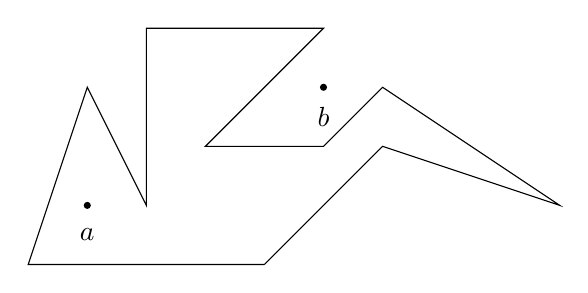
\begin{tikzpicture}[scale=0.75]
%\draw (0,0)--(2,-2)--(3,1)--(5,1)--(2,3)--(1,2)--(-1,2)--(1,4)--(-2,4)--(-2,1)--(-3,3)--(-4,0)--(0,0);
\draw (0,0)--(2,2)--(5,1)--(2,3)--(1,2)--(-1,2)--(1,4)--(-2,4)--(-2,1)--(-3,3)--(-4,0)--(0,0);

\draw[fill] (-3,1) circle [radius=0.05];
\node at (-3,0.5) {$a$};
\draw[fill] (1,3) circle [radius=0.05];
\node at (1,2.5) {$b$};
\end{tikzpicture}
\end{center}

Kätevä ratkaisu tehtävään
on lähettää pisteestä säde
satunnaiseen suuntaan ja laskea,
montako kertaa se osuu monikulmion reunaan.
Jos kertoja on pariton määrä,
niin piste on sisäpuolella,
ja jos taas kertoja on parillinen määrä,
niin piste on ulkopuolella.

\begin{samepage}
Äskeisessä tilanteessa säteitä
voisi lähteä seuraavasti:
\begin{center}
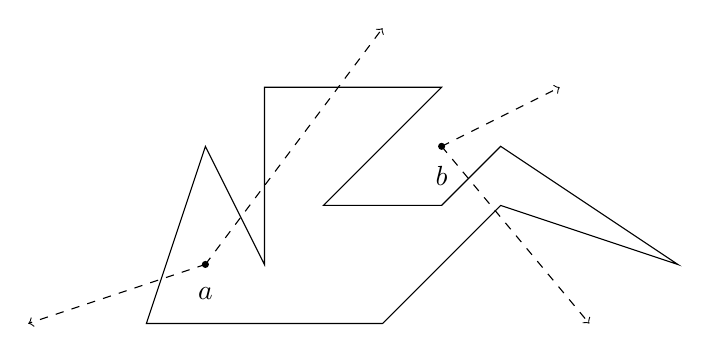
\begin{tikzpicture}[scale=0.75]
\draw (0,0)--(2,2)--(5,1)--(2,3)--(1,2)--(-1,2)--(1,4)--(-2,4)--(-2,1)--(-3,3)--(-4,0)--(0,0);

\draw[fill] (-3,1) circle [radius=0.05];
\node at (-3,0.5) {$a$};
\draw[fill] (1,3) circle [radius=0.05];
\node at (1,2.5) {$b$};

\draw[dashed,->] (-3,1)--(-6,0);
\draw[dashed,->] (-3,1)--(0,5);

\draw[dashed,->] (1,3)--(3.5,0);
\draw[dashed,->] (1,3)--(3,4);
\end{tikzpicture}
\end{center}
\end{samepage}

Pisteestä $a$ lähtevät säteet osuvat 1 ja 3
kertaa monikulmion reunaan,
joten piste on sisäpuolella.
Vastaavasti pisteestä $b$ lähtevät
säteet osuvat 0 ja 2 kertaa monikulmion reunaan,
joten piste on ulkopuolella.

\section{Monikulmion pinta-ala}

Yleinen kaava monikulmion pinta-alan laskemiseen on
\[\frac{1}{2} |\sum_{i=1}^{n-1} (p_i \times p_{i+1})| =
\frac{1}{2} |\sum_{i=1}^{n-1} (x_i y_{i+1} - x_{i+1} y_i)|, \]
kun kärkipisteet ovat
$p_1=(x_1,y_1)$, $p_2=(x_2,y_2)$, $\ldots$, $p_n=(x_n,y_n)$
järjestettynä niin,
että $p_i$ ja $p_{i+1}$ ovat vierekkäiset kärkipisteet
monikulmion reunalla
ja ensimmäinen ja viimeinen kärkipiste ovat samat eli $p_1=p_n$.

Esimerkiksi monikulmion
\begin{center}
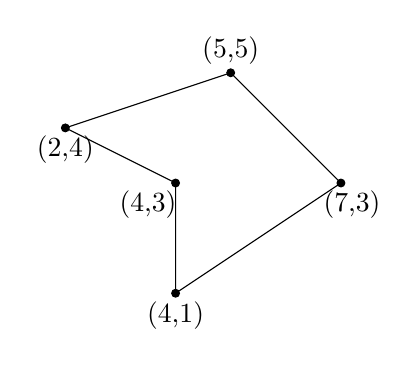
\begin{tikzpicture}[scale=0.7]
\filldraw (4,1.4) circle (2pt);
\filldraw (7,3.4) circle (2pt);
\filldraw (5,5.4) circle (2pt);
\filldraw (2,4.4) circle (2pt);
\filldraw (4,3.4) circle (2pt);
\node (1) at (4,1) {(4,1)};
\node (2) at (7.2,3) {(7,3)};
\node (3) at (5,5.8) {(5,5)};
\node (4) at (2,4) {(2,4)};
\node (5) at (3.5,3) {(4,3)};
\path[draw] (4,1.4) -- (7,3.4) -- (5,5.4) -- (2,4.4) -- (4,3.4) -- (4,1.4);
\end{tikzpicture}
\end{center}
pinta-ala on
\[\frac{|(2\cdot5-4\cdot5)+(5\cdot3-5\cdot7)+(7\cdot1-3\cdot4)+(4\cdot3-1\cdot4)+(4\cdot4-3\cdot2)|}{2} = 17/2.\]
Kaavassa on ideana käydä läpi puolisuunnikkaita,
joiden yläreuna on yksi monikulmion sivuista ja
alareuna on vaakataso. Esimerkiksi:
\begin{center}
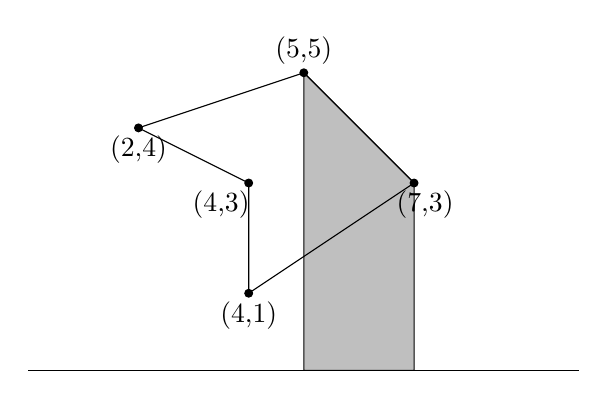
\begin{tikzpicture}[scale=0.7]
\path[draw,fill=lightgray] (5,5.4) -- (7,3.4) -- (7,0) -- (5,0) -- (5,5.4);
\filldraw (4,1.4) circle (2pt);
\filldraw (7,3.4) circle (2pt);
\filldraw (5,5.4) circle (2pt);
\filldraw (2,4.4) circle (2pt);
\filldraw (4,3.4) circle (2pt);
\node (1) at (4,1) {(4,1)};
\node (2) at (7.2,3) {(7,3)};
\node (3) at (5,5.8) {(5,5)};
\node (4) at (2,4) {(2,4)};
\node (5) at (3.5,3) {(4,3)};
\path[draw] (4,1.4) -- (7,3.4) -- (5,5.4) -- (2,4.4) -- (4,3.4) -- (4,1.4);
\draw (0,0) -- (10,0);
\end{tikzpicture}
\end{center}
Tällaisen puolisuunnikkaan pinta-ala on
\[(x_{i+1}-x_{i}) \frac{y_i+y_{i+1}}{2},\]
kun kärkipisteet ovat $p_i$ ja $p_{i+1}$.
Jos $x_{i+1}>x_{i}$, niin pinta-ala on positiivinen,
ja jos $x_{i+1}<x_{i}$, niin pinta-ala on negatiivinen.

Monikulmion pinta-ala saadaan laskemalla yhteen kaikkien
tällaisten puolisuunnikkaiden pinta-alat, mistä tulee:

\[|\sum_{i=1}^{n-1} (x_{i+1}-x_{i}) \frac{y_i+y_{i+1}}{2}| =
\frac{1}{2} |\sum_{i=1}^{n-1} (x_i y_{i+1} - x_{i+1} y_i)|.\]

Huomaa, että pinta-alan kaavassa on itseisarvo,
koska monikulmion kiertosuunnasta (myötä- tai vastapäivään)
riippuen tuloksena oleva pinta-ala on joko
positiivinen tai negatiivinen.

\subsubsection{Pickin lause}

\index{Pickin lause}

Pickin lause on vaihtoehtoinen tapa laskea
monikulmion pinta-ala,
kun kaikki monikulmion kärkipisteet
ovat kokonaislukupisteissä.
Pickin lauseen mukaan monikulmion pinta-ala on
\[ a + b/2 -1,\]
missä $a$ on kokonaislukupisteiden määrä monikulmion sisällä
ja $b$ on kokonaislukupisteiden määrä monikulmion reunalla.

Esimerkiksi monikulmion
\begin{center}
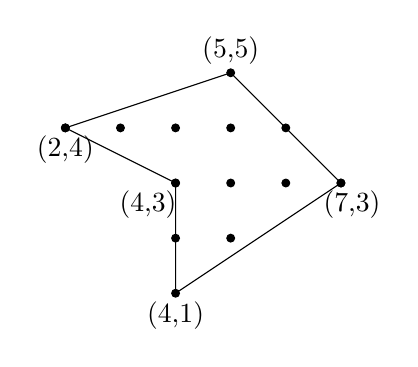
\begin{tikzpicture}[scale=0.7]
\filldraw (4,1.4) circle (2pt);
\filldraw (7,3.4) circle (2pt);
\filldraw (5,5.4) circle (2pt);
\filldraw (2,4.4) circle (2pt);
\filldraw (4,3.4) circle (2pt);
\node (1) at (4,1) {(4,1)};
\node (2) at (7.2,3) {(7,3)};
\node (3) at (5,5.8) {(5,5)};
\node (4) at (2,4) {(2,4)};
\node (5) at (3.5,3) {(4,3)};
\path[draw] (4,1.4) -- (7,3.4) -- (5,5.4) -- (2,4.4) -- (4,3.4) -- (4,1.4);

\filldraw (2,4.4) circle (2pt);
\filldraw (3,4.4) circle (2pt);
\filldraw (4,4.4) circle (2pt);
\filldraw (5,4.4) circle (2pt);
\filldraw (6,4.4) circle (2pt);

\filldraw (4,3.4) circle (2pt);
\filldraw (5,3.4) circle (2pt);
\filldraw (6,3.4) circle (2pt);
\filldraw (7,3.4) circle (2pt);

\filldraw (4,2.4) circle (2pt);
\filldraw (5,2.4) circle (2pt);
\end{tikzpicture}
\end{center}

pinta-ala on $6+7/2-1=17/2$.

